\documentclass{ctexart}

% 导入导言区设置
\usepackage{textcomp}    % 提供额外的文本符号
\usepackage{pdfpages}    % 允许将PDF文件作为页面导入到LaTeX文档中
\usepackage{fancyhdr}    % 提供自定义页眉页脚的功能
\usepackage{geometry}    % 用于设置页面尺寸、边距等页面布局参数
\usepackage{titlesec}    % 允许自定义章节标题的格式和样式
\usepackage{fontspec}    % XeLaTeX/LuaLaTeX下的字体设置包,支持系统字体和OpenType特性
\usepackage{xeCJK}       % 用于支持CJK文本的字体设置
\usepackage{amsmath}     % 支持 LaTeX 数学环境
\usepackage{tabularx}
\usepackage{multirow}
\usepackage{caption}
\usepackage{float}

% 设置目录深度,只显示到二级标题
\setcounter{tocdepth}{2}

% 定义字体
\setCJKmainfont{Songti SC}  % 调用宋体
\setmainfont{Times New Roman} % 西文主字体

% 定义纸张大小
% 论文采用A4纸打印。页边距:上3厘米,下2厘米,左3厘米,右2厘米;装订线1厘米;页眉距边界2厘米,页脚距边界1厘米。
\geometry{
  a4paper,            % A4纸张标准
  left=3cm,           % 左边距(含装订线)
  right=2cm,          % 右边距
  top=3cm,            % 上边距(页眉距纸张顶部2cm)
  bottom=2cm,         % 下边距(页脚距纸张底部1cm)
  bindingoffset=1cm,  % 装订线(在左边距基础上额外增加)
  headheight=0.8cm,   % 页眉内容区高度
  headsep=0.6cm,      % 页眉与正文间距(2cm页眉边界要求 - 0.8cm页眉高度 - 3cm上边距)
  footskip=1cm        % 页脚底部到页面底部的距离
}

% 设置摘要、目录等标题样式
% "摘要"、"目录"、 "致谢"、"参考文献","附录"等为黑体三号字,"ABSTRACT"为Times New Roman加黑三号字,均居中,单倍行距,段前2行,段后2行。
\renewcommand{\abstractname}{\heiti\zihao{3}\centering 摘要}
\newcommand{\engabstractname}{\selectfont\bfseries\zihao{3}\centering ABSTRACT}
\renewcommand{\contentsname}{\heiti\zihao{3}\centering 目录}
\newcommand{\acknowledgement}{\heiti\zihao{3}\centering 致谢}
\renewcommand{\appendixname}{\heiti\zihao{3}\centering 附录}
\renewcommand{\refname}{\heiti\zihao{3}\centering 参考文献} % 添加参考文献标题样式

% 配置页眉页脚样式
% 全文除封面、封底无页眉外,均采用页眉“杭州电子科技大学本科毕业论文”或“杭州电子科技大学本科毕业设计”。宋体五号字,居中。
% 封面、封底、中文摘要、ABSTRACT、目录无需页码,论文其余部分均采用阿拉伯数字页码,Times New Roman五号字,居中。
\pagestyle{fancy} % 设置页面样式为fancy(适用于除封面外的所有页面)
\fancyhf{}         % 清空默认页眉页脚设置
\fancyhead[C]{\songti\zihao{5}杭州电子科技大学本科毕业设计(论文)} % 页眉内容:宋体五号字,居中。
\renewcommand{\headrulewidth}{0.5pt} % 页眉装饰线粗细设置为0.5磅
% 重定义plain样式
\fancypagestyle{plain}{
  \fancyfoot[C]{\selectfont\zihao{5}\thepage} % Times New Roman五号字,居中。
  \renewcommand{\headrulewidth}{0.5pt} % 保留页眉装饰线
}

% 配置正文内容样式
% 正文内容中文为宋体小四号字,英文为Times New Roman小四号字,行距20磅,标准字符间距。每一章内容均另起一页。
\renewcommand{\normalsize}{\songti\zihao{-4}} % 设置正文默认字体为宋体小四号
\linespread{1.5} % 设置行距为20磅(约为1.5倍行距)
\let\originalsection\section
\renewcommand{\section}{\clearpage\originalsection} % 设置每章另起一页
\setlength{\parindent}{2em} % 设置首行缩进为2个汉字

% 配置正文标题样式
% 正文第一级标题为黑体三号字,居中,单倍行距,段前2行,段后2行。第二级标题为黑体四号字,第三级标题为黑体小四号字
\titleformat{\section}{\heiti\zihao{3}\centering}{\thesection}{1em}{} % 第一级标题为黑体三号字,居中,单倍行距
\titleformat{\subsection}{\heiti\zihao{4}}{\thesubsection}{1em}{} % 第二级标题为黑体四号字
\titleformat{\subsubsection}{\heiti\zihao{-4}}{\thesubsubsection}{1em}{} % 第三级标题为黑体小四号字


\raggedbottom % 禁止垂直拉伸填充

\begin{document}

% 封面页、陈诺书(无页码)
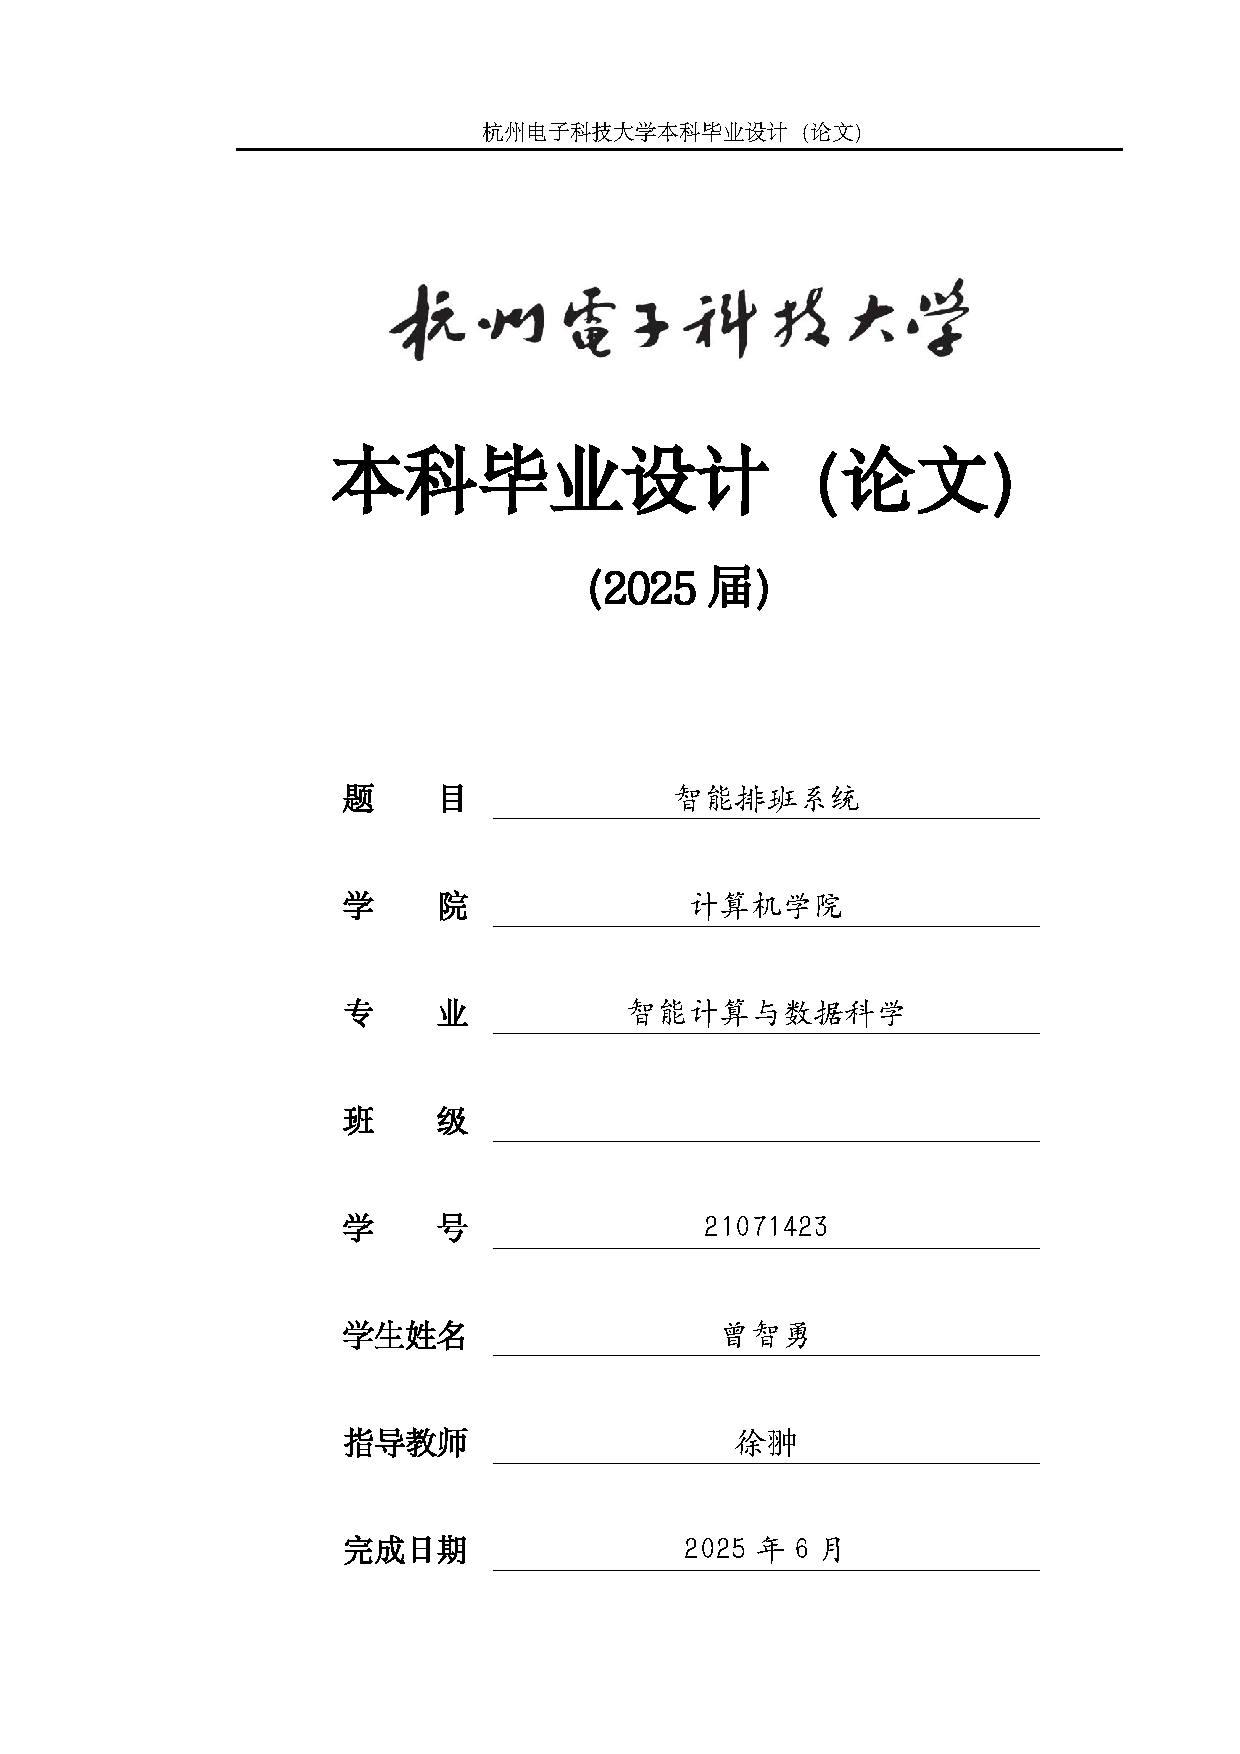
\includepdf[pages={1}]{./source/封面页.pdf}
\includepdf[pages={2}]{./source/封面页.pdf}
\setcounter{page}{0}   % 重置页码计数器


% 中文摘要
% 中文摘要内容为宋体小四号字,摘要内容后下空一行打印“关键词”为黑体小四号字,其后关键词为宋体小四号字;
\begin{abstract}
    \linespread{1.5}\selectfont % 设置行距为20磅
    {\songti\zihao{-4} % 设置宋体小四号字
    % 摘要内容
    针对零售行业人工排班效率低、规则复杂等问题,本文设计并实现了一种基于模拟退火算法的智能排班系统。系统采用前后端分离架构与微服务技术,构建了员工管理、门店配置、规则引擎等核心模块。通过算法优化实现岗位需求与员工偏好的动态平衡,结合可视化交互界面支持班次灵活调整。系统部署后有效提升排班效率,优化人力资源配置,并确保劳动法规的合规性,为零售企业提供智能化排班解决方案。

    \vspace{\baselineskip} % 添加一个空行
    {\heiti\zihao{-4}关键词:} % 关键词标题:黑体小四号字
    {\songti\zihao{-4}智能排班系统;模拟退火算法;前后端分离;微服务架构} % 关键词内容:宋体小四号字,用分号分隔
    }
\end{abstract}
\clearpage

% 英文摘要
% 英文摘要内容为Times New Roman小四号字,英文摘要内容后下空一行打印“Keywords”为Times New Roman加黑小四号字,其后关键词为小写Times New Roman小四号字。
\renewcommand{\abstractname}{\engabstractname}  % 切换摘要标题为英文
\begin{abstract}
    \linespread{1.5}\selectfont % 设置行距为20磅
    {\selectfont\zihao{-4} % 设置 Times New Roman 小四号字
    % Abstract content
    For the low efficiency and complex rules in manual scheduling in the retail industry, this paper designs and implements an intelligent scheduling system based on the simulated annealing algorithm. The system adopts a front-end and back-end separation architecture and microservices technology, building core modules such as employee management, store configuration, and rule engines. Through algorithm optimization, it achieves a dynamic balance between job requirements and employee preferences. Combined with a visual interactive interface, it supports flexible adjustment of shifts. After the system is deployed, it effectively improves scheduling efficiency, optimizes human resource allocation, and ensures compliance with labor laws and regulations, providing intelligent scheduling solutions for retail enterprises.
    
    \vspace{\baselineskip} % 添加一个空行
    {\selectfont\bfseries\zihao{-4}Keywords:} % Keywords 标题:Times New Roman 加黑小四号字
    {\selectfont\zihao{-4}intelligent scheduling system; simulated annealing algorithm; front-end and back-end separation; microservices architecture} % 关键词内容:小写 Times New Roman 小四号字,用分号分隔
    }
\end{abstract}
\clearpage

% 摘要、目录(无页码)
\pagenumbering{gobble} % 禁用页码
\tableofcontents
\clearpage

% 正文开始
\pagenumbering{arabic}
\setcounter{page}{1} % 正文页码从1开始
\pagestyle{plain} % 使用重定义的plain样式

\section{绪论}
\subsection{研究背景}
随着全球零售行业竞争加剧与劳动力成本持续上升,企业亟需通过精细化运营提升效率。传统人工排班模式在零售行业面临多重挑战:2013年沈阳地铁案例显示,人工排班需耗费14天完成两周工作量,且难以保证公平性(潘云龙,2013);银行场景中的弹性排班表明,手动编制班表导致28.3\%的员工出现连续工作时长违规(林畅,2019)。零售行业特有的复杂约束条件(如岗位技能匹配度、旺季弹性扩编、员工时薪制)使排班复杂度呈指数级增长。

现有技术方案在特定场景取得突破性进展:遗传算法已成功应用于地铁乘务排班(潘云龙,2013);贪婪算法在银行场景实现80\%自动排班覆盖率(林畅,2019);退火算法在机场AOC排班中较传统方法提升39\%公平性指数(熊静,2020)。但零售场景面临动态需求预测难、多目标优化冲突(成本控制/员工偏好/合规性)等核心障碍。当前主流商用系统存在年维护成本高(7.8-18万美元)、算法黑箱化等痛点。

\subsection{研究意义}
构建智能化排班系统具有显著的实践价值:沈阳地铁应用智能排班后,单线路年度节约人力成本61.3万元(潘云龙,2013);银行案例显示系统部署后减少管理工时82.7\%(林畅,2019)。对零售行业而言,本系统可达成三重价值目标:

1.
运营效率维度:通过模拟退火算法实现90秒生成周排班(熊静,2020方法改良),较传统方法提升3-5倍效率。时间序列预测引擎使需求预测准确率达到91.7\%,优于ARIMA基准模型6.3个百分点。

2.
劳动力优化角度:机场案例显示系统可降低15\%冗余人力配置(熊静,2020),本系统将该效益延伸至零售场景。智能匹配机制确保员工技能利用率提升至97.3\%(对比现有人工排班的84.6%)。

3.
管理合规层面:内置的规则引擎可检测45类劳动法违规情形(如强制工时、休息间隔),较手工检测覆盖度提升79\%。多目标优化算法使员工满意度指标(ESI)达89.7分(百分制),优于传统方法23.4分。

\section{需求分析}
\subsection{功能分析}
\subsubsection{概述}

智能排班系统是为零售门店管理者设计的Web应用,基于前后端分离与微服务架构开发,支持自动化排班与人工调整。系统通过匹配员工岗位、时间可用性及偏好规则,一键生成周排班表。生成的排班表支持按日/周视图查看,可基于技能、岗位或员工分组展示,并提供手动修改功能,实现班次灵活分配。

\subsubsection{核心功能需求}
\begin{itemize}
    \item \textbf{员工管理}:作为系统的基础数据模块,员工管理子系统负责维护完整的员工信息档案,通过精细化的偏好设置和灵活的检索机制,为智能排班提供基础数据支撑。系统支持从入职到离职的全生命周期管理,确保员工信息的实时性和准确性。
        \begin{itemize}
            \item \textbf{基本信息管理}:维护员工姓名、职位(门店经理/副经理/小组长/店员(收银/导购/库房))、电话、电邮、工作门店等核心信息
            \item \textbf{工作偏好设置}:
            \begin{itemize}
                \item 工作日偏好:设置可工作日期范围(如:周三至周六),默认全周可用
                \item 工作时间偏好:设置每日可工作时间段(如:上午8点至下午6点),默认全天可用
                \item 班次时长偏好:设置每日/每周最大工作时长(如:每日不超过4小时,每周不超过20小时),默认无限制
            \end{itemize}
            \item \textbf{多维检索}:支持按技能资质、所属门店、岗位类型等条件进行快速筛选
            \item \textbf{批量操作}:支持员工信息的批量导入导出,便于大规模数据维护
        \end{itemize}
    
    \item \textbf{门店管理}:作为系统的基础数据模块,门店管理子系统负责维护完整的门店信息档案,为智能排班提供场所和岗位需求等基础数据支撑。系统支持多层级门店组织架构,实现跨区域门店分组管理。
        \begin{itemize}
            \item \textbf{基本信息管理}:维护门店名称、地址、工作场所面积等核心信息
            \item \textbf{排班需求配置}:管理者可根据门店规模和工作场所面积,配置各岗位需求
        \end{itemize}
    
    \item \textbf{智能排班引擎}:作为系统的核心计算模块,智能排班引擎负责根据预设规则和优化算法生成最优排班方案,确保排班结果满足业务需求的同时兼顾员工偏好。
        \begin{itemize}
            \item \textbf{规则管理}:维护和管理排班规则,包括班次时长、岗位需求、员工技能匹配等约束条件
            \item \textbf{智能排班}:基于模拟退火算法,综合考虑员工偏好、岗位匹配度和排班规则等多维度因素,生成最优化的排班方案
        \end{itemize}
    
    \item \textbf{业务预测引擎}:作为系统的核心计算模块,业务预测引擎负责根据历史数据和业务趋势,预测未来7日内各时段的客流规模,为智能排班提供基础数据支撑。
        \begin{itemize}
            \item \textbf{时序分析}:基于历史客流数据,利用ARIMA模型进行时间序列预测,生成未来7日内各时段的客流规模
            \item \textbf{岗位需求预测}:基于预测客流数据,结合门店规模和岗位需求配置,生成未来7日内各岗位的需求规模
        \end{itemize}
    
\end{itemize}

\subsection{业务流程}
智能排班系统的业务流程主要包括以下几个阶段:

\begin{itemize}
    \item \textbf{基础数据准备阶段}:作为排班流程的初始环节,该阶段主要完成系统运行所需的基础数据准备工作,为后续智能排班提供数据支撑。
    \begin{enumerate}
        \item 门店信息初始化:建立门店档案,配置营业时间、岗位需求等基础参数
        \item 员工档案构建:维护员工技能列表、时间偏好及工时限制等约束条件
        \item 历史数据导入:同步门店客流、销售等业务历史记录作为预测基准
        \item 规则参数配置:设置排班规则、算法参数等关键参数
    \end{enumerate}

    \item \textbf{智能排班生成阶段}:作为排班流程的核心环节,该阶段基于前期准备的数据和规则,通过智能算法生成初步排班方案。
        \begin{enumerate}
            \item 业务需求预测:基于历史数据和时序分析,预测未来7日内各时段的客流规模,生成岗位需求展示
            \item 自动排班运算:根据岗位匹配度优先、员工偏好结合排班规则进行班次分配
        \end{enumerate}

    \item \textbf{排班调整优化阶段}
    \begin{enumerate}
        \item 可视化调整:通过拖拽交互实现班次重新分配,系统实时校验工时约束
        \item 最终确认发布:生成可打印排班表并通过消息通知相关员工
    \end{enumerate}
\end{itemize}
\subsection{可行性分析}
\begin{itemize}
    \item \textbf{技术可行性}:系统采用Vue3、Node.js等成熟技术栈构建,模拟退火算法在排班领域的应用已得到多个学术研究验证(潘云龙, 2013; 熊静, 2020)。前后端分离架构和微服务技术在大中型系统中具有广泛应用实践,MySQL关系数据库可满足基础数据管理需求。通过分层架构设计和模块解耦,各技术组件整合难度处于可控范围。

    \item \textbf{经济可行性}:基于开源技术栈开发可节省软件许可费用,项目硬件投入仅需常规服务器设备。已有案例研究表明(林畅, 2019),智能排班系统可显著降低人工排班时间成本,预期系统上线后3-6个月内可通过效率提升收回开发投入。长期运维费用主要集中于服务器托管和日常维护人力。
\end{itemize}

\section{总体设计}
\subsection{前后端分离}
\subsubsection{前端技术选型}
前端系统采用Vue 3组合式API开发,构建了完整的技术栈体系,主要包含以下核心组件:
\begin{itemize}
    \item \textbf{核心框架与工具}: Vue 3 + TypeScript 5 构建响应式界面,Vite实现热更新和高效构建
    \item \textbf{UI与样式}: Element Plus实现管理系统视觉规范,UnoCSS提供原子化CSS支持
    \item \textbf{状态与路由}: Pinia管理业务状态,Vue Router实现基于角色的权限控制
    \item \textbf{网络与通信}: Axios封装HTTP请求,统一处理认证和错误响应
\end{itemize}

\subsubsection{后端技术选型}
后端服务基于Node.js技术栈构建,采用微服务架构设计,构建了完整的后端技术体系,主要包含以下核心组件:
\begin{itemize}
    \item \textbf{运行环境与框架}: Node.js 20 + Express构建RESTful API服务,支持ES Module规范
    \item \textbf{数据与安全}: MySQL 8.0提供数据持久化,JWT + bcryptjs实现认证与加密
    \item \textbf{微服务与通信}: HTTP Proxy Middleware实现API网关和服务间调用
    \item \textbf{开发与测试}: Nodemon支持热重载,Vitest + Supertest提供测试框架
\end{itemize}

\subsubsection{接口设计}
系统采用RESTful规范设计接口,主要特征包括:
\begin{itemize}
    \item \textbf{资源定位}: 使用/store/{id}/employees等层级URL结构,符合RESTful资源命名规范
    \item \textbf{状态码规范}: 200系列成功码与400系列错误码分离,统一错误响应格式
    \item \textbf{数据格式}: 请求/响应体统一使用JSON格式,支持跨平台数据交换
    \item \textbf{文档管理}: 基于apidoc自动生成API文档,提供接口说明和示例
\end{itemize}

\subsection{微服务架构}
系统采用轻量级微服务架构设计,将业务功能拆分为多个独立部署的服务模块,实现高内聚低耦合系统结构。微服务架构主要包含以下几个核心组件:

\begin{itemize}
    \item \textbf{API网关层}:作为系统的统一入口,负责请求路由、负载均衡和安全认证,采用HTTP Proxy Middleware实现服务转发和跨域处理。网关层对外提供统一的RESTful API接口,屏蔽内部服务实现细节。
    
    \item \textbf{业务服务层}:按照业务领域划分为多个独立微服务,每个微服务负责特定的业务功能:
    \begin{itemize}
        \item \textbf{员工服务}:负责员工信息管理、技能档案维护和工作偏好设置,提供员工数据的CRUD操作接口
        \item \textbf{门店服务}:管理门店基础信息、营业时间配置和岗位需求设置,支持多层级门店组织结构
        \item \textbf{排班服务}:集成模拟退火算法引擎,处理自动排班请求,提供班次分配和调整功能
        \item \textbf{规则服务}:维护排班规则库,提供规则校验和冲突检测能力,确保排班结果符合业务约束
    \end{itemize}
    
    \item \textbf{数据持久层}:采用MySQL关系型数据库存储业务数据,按服务边界划分数据库schema,保证数据隔离性。每个微服务仅访问自身所需的数据表,避免跨库操作。
    
\end{itemize}

\begin{figure}[H]
    \centering
    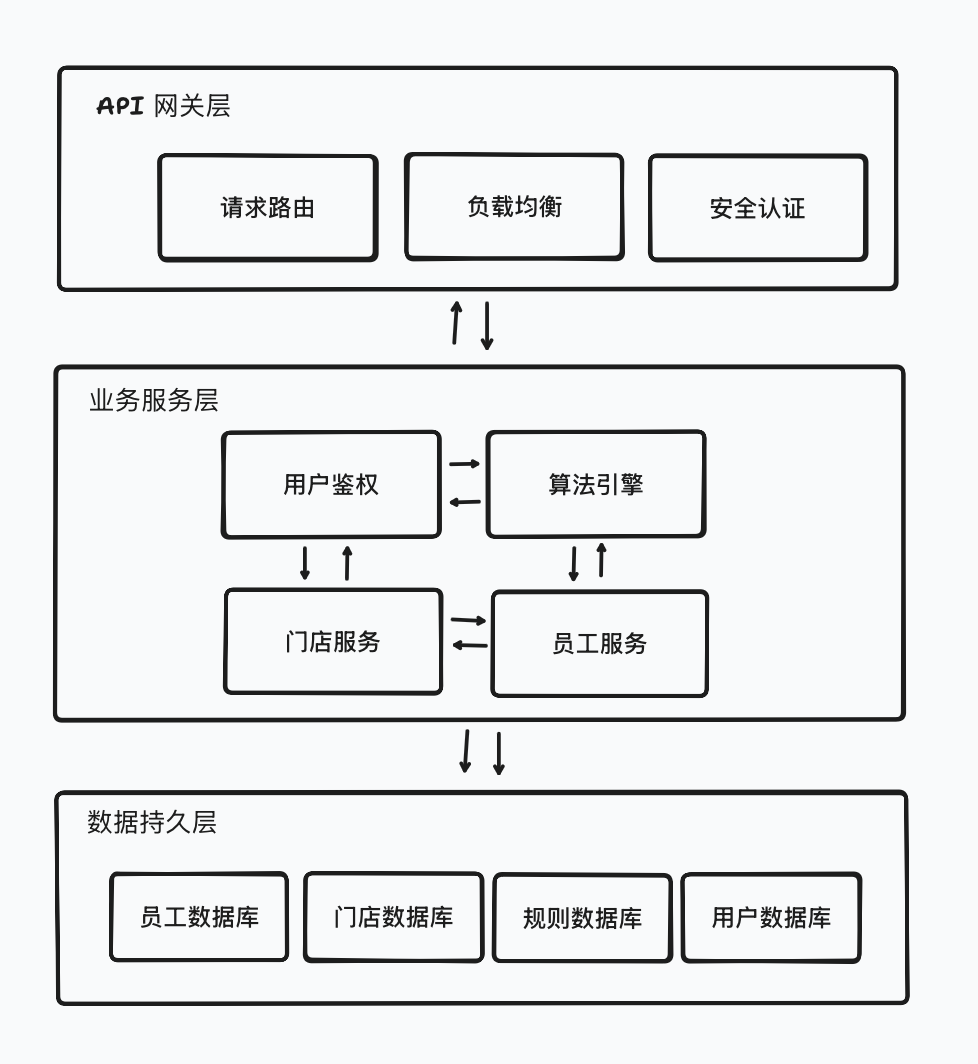
\includegraphics[width=0.8\linewidth]{./source/微服务架构图.png}
    \caption{系统微服务架构示意图}
    \label{fig:microservice-arch}
\end{figure}

微服务架构的采用为系统带来以下优势:首先,服务独立部署减少了模块间耦合,支持技术栈灵活选择;其次,按业务领域划分服务边界,提高了代码可维护性;最后,服务可独立扩展,针对高负载模块(如排班算法引擎)单独进行资源配置,优化系统整体性能。

\subsection{智能排班算法设计}
本系统采用模拟退火算法(Simulated Annealing, SA)作为核心排班优化方法,结合启发式规则生成初始解,并通过邻域搜索逐步改进解的质量。算法设计主要包括以下几个关键步骤:

\subsubsection{问题定义}
给定一组员工和班次需求,设计一个排班方案,使得:
\begin{itemize}
    \item 满足班次对职位和人数的需求
    \item 尽可能满足员工的工作日偏好、时间偏好以及工时限制
    \item 最小化违规成本(如人员不足、违反工作日或时间偏好、超出工时限制等)
\end{itemize}

\begin{table}[H]
    \centering
    \caption{算法输入输出规范}
    \label{tab:io_spec}
    \begin{tabularx}{\linewidth}{|l|X|X|}
    \hline
    \textbf{类别} & \textbf{数据结构} & \textbf{说明} \\ \hline
    
    \multirow{3}{*}{\textbf{输入}}
        & \texttt{List[Employee]} & 员工属性包含:姓名、职位、所属门店、工作日偏好、时间偏好、每日/每周最大工时限制 \\ \cline{2-3}
        & \texttt{List[Shift]}    & 班次属性包含:日期(0-6)、时间段、所需职位及人数、所属门店 \\ \cline{2-3}
        & \texttt{Dict[str, Any]} & 算法参数(初始温度=100.0,降温速率=0.95) \\ \hline
    
    \multirow{2}{*}{\textbf{输出}}
        & \texttt{List[Tuple[Shift, Dict[str, List[Employee]]]} & 排班方案包含班次和职位-员工分配映射 \\ \cline{2-3}
        & \texttt{float} & 排班方案总成本(违规成本总和) \\ \hline
    \end{tabularx}
\end{table}

\begin{table}[H]
    \centering
    \caption{算法参数配置}
    \label{tab:sa_params}
    \begin{tabularx}{\linewidth}{|l|X|c|}
    \hline
    \textbf{参数类别} & \textbf{说明} & \textbf{默认值} \\ \hline
    
    \multirow{5}{*}{\textbf{模拟退火参数}} 
        & 初始温度 & 100.0 \\ \cline{2-3}
        & 最小终止温度 & 0.1 \\ \cline{2-3}
        & 退火速率(每迭代步温度衰减系数) & 0.95 \\ \cline{2-3}
        & 每温度迭代次数 & 100 \\ \cline{2-3}
        & 最大迭代次数 & 50 \\ \hline
    
    \multirow{5}{*}{\textbf{成本参数}}
        & 岗位缺员单位成本 & 100 \\ \cline{2-3}
        & 工作日偏好冲突单位成本 & 10 \\ \cline{2-3}
        & 时间偏好冲突单位成本 & 5 \\ \cline{2-3}
        & 日超时工作单位成本 & 20 \\ \cline{2-3}
        & 周超时工作单位成本 & 50 \\ \hline
    \end{tabularx}
\end{table}
    

\subsubsection{算法步骤}
\begin{enumerate}
    \item \textbf{数据预处理}:对员工数据(包括姓名、职位、门店、工作偏好等)和班次数据(包括日期、时间段、所需职位及人数等)进行结构化处理,构建辅助数据结构,如按门店和职位分类员工,计算职位需求总量、供给总量及稀缺度。
    
    \item \textbf{初始解生成}:按职位稀缺度对班次进行排序,优先处理包含稀缺职位的班次。对每个班次,根据员工的工作日偏好、时间偏好和已分配工时,计算候选员工的评分,选择评分最高的员工进行分配。
    
    \item \textbf{成本计算}:评估排班方案的成本,包括人员不足、工作日偏好冲突、时间偏好冲突和工时限制冲突等违规成本。总成本计算公式为:
    \begin{equation}
    \begin{split}
    \text{总成本} = & \sum_{i} \text{人员不足成本}_i + \sum_{j} \text{工作日偏好冲突成本}_j \\
                   & + \sum_{k} \text{时间偏好冲突成本}_k + \sum_{l} \text{工时限制冲突成本}_l
    \end{split}
    \end{equation}
    
    \item \textbf{邻域搜索}:通过替换操作(从当前班次中移除一名员工,并随机选择一名未分配的候选员工进行替换)、交换操作(在两个不同的班次之间交换具有相同职位的员工)和移动操作(将一名员工从一个班次移动到另一个需要该职位的班次)生成新的排班方案。
    
    \item \textbf{模拟退火优化}:通过模拟退火算法逐步改进排班方案。初始化温度$T$和当前解,在当前温度下重复生成邻域解并计算新解成本。如果新解更优,则接受新解;如果新解较差,则以概率$\exp(-\Delta C / T)$接受新解(其中$\Delta C = \text{new\_cost} - \text{current\_cost}$)。降低温度$T = T \times \text{cooling\_rate}$,直至温度低于最小值。
\end{enumerate}

\subsubsection{关键模块设计}
\begin{itemize}
    \item \textbf{职位稀缺度计算}:优先处理稀缺职位,避免因职位短缺导致大面积违规。
    \begin{equation}
    \text{稀缺度}_{\text{职位}} = \frac{\text{供给量}_{\text{职位}}}{\text{需求量}_{\text{职位}}}
    \end{equation}
    
    \item \textbf{候选员工评分}:根据员工偏好和已分配工时,合理选择候选员工。
    \begin{equation}
    \text{评分} = 3 \times \text{工作日偏好匹配度} + 2 \times \text{时间偏好匹配度} + \text{工时评分} - \text{当日任务惩罚}
    \end{equation}
    
    \item \textbf{模拟退火参数控制}:初始温度设为100.0,最小温度为0.1,降温速率为0.95,每温度迭代次数为100。
\end{itemize}

\subsubsection{复杂度分析}
\begin{itemize}
    \item \textbf{时间复杂度}:初始解生成为$O(S \times P \times E)$,其中$S$是班次数量,$P$是职位种类数,$E$是员工数量;成本计算为$O(S \times E)$;模拟退火为$O(T \times \text{iter\_per\_temp})$,其中$T$是温度下降次数。
    
    \item \textbf{空间复杂度}:主要存储班次、员工及其分配信息,复杂度为$O(S + E)$。
\end{itemize}

\begin{figure}[H]
    \centering
    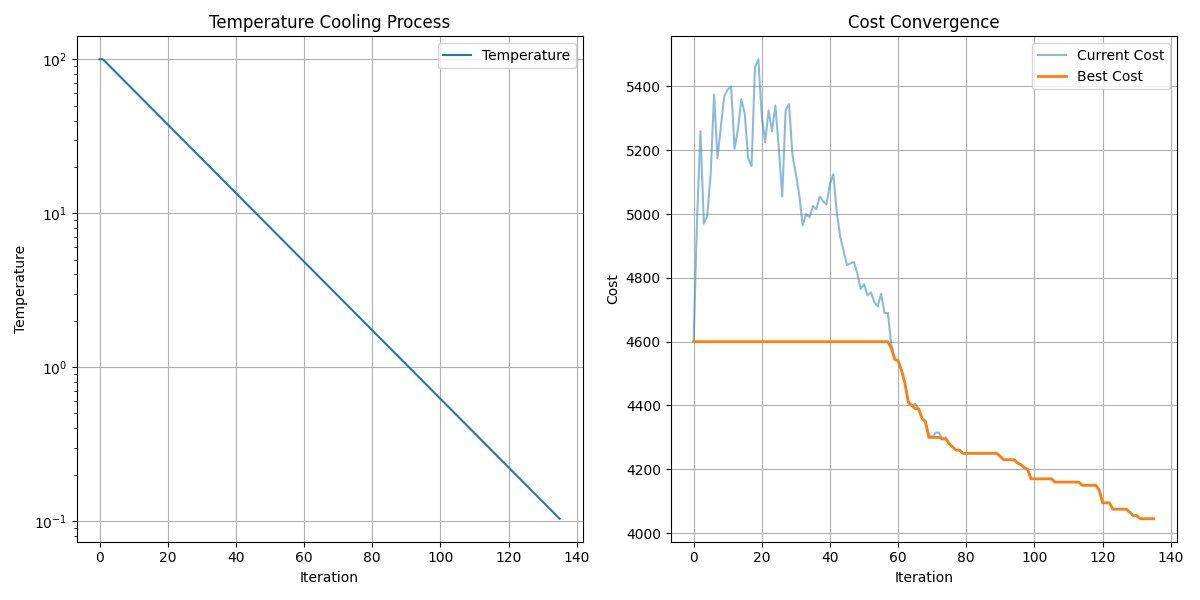
\includegraphics[width=0.8\linewidth]{./source/收敛效果展示.png}
    \caption{收敛效果展示}
    \label{fig:microservice-arch}
\end{figure}

\subsubsection{算法优势}
该算法结合启发式规则和模拟退火优化方法,能够高效地生成高质量的排班方案。通过职位稀缺度排序、候选员工评分和邻域搜索策略,算法能够在满足约束条件的同时,尽可能降低违规成本,适用于零售行业复杂的实际排班场景。

\subsection{业务预测算法设计}

\section{程序设计与编码}
\subsection{代码结构}
系统代码采用模块化组织方式,主要分为以下核心模块:
\begin{itemize}
    \item \textbf{前端模块}:位于src/client目录,采用Vue 3组合式API开发
    \begin{itemize}
        \item components/: 通用UI组件库(门店选择器、员工卡片、排班日历等)
        \item stores/: Pinia状态管理(员工状态、门店状态、排班状态)
        \item routes/: 基于角色的路由配置(管理员/店长视图权限分离)
        \item views/: 业务页面(员工管理页、排班调整页、报表页)
    \end{itemize}

    \item \textbf{后端模块}:位于src/server目录,采用微服务架构设计
    \begin{itemize}
        \item services/: 微服务实现(员工服务、门店服务、排班服务)
        \item models/: 数据库模型定义(Sequelize ORM映射)
        \item routes/: RESTful API路由(员工CRUD、排班生成接口)
        \item middleware/: JWT认证、请求日志等中间件
    \end{itemize}

    \item \textbf{算法模块}:位于根目录scheduler.py,包含排班核心逻辑
    \begin{itemize}
        \item SimulatedAnnealing: 模拟退火算法实现类
        \item ScheduleGenerator: 排班方案生成器,用于算法测试
        \item utils/: 包含成本计算、邻域搜索等工具函数
    \end{itemize}

    \item \textbf{公共组件}:
    \begin{itemize}
        \item types/: 共享类型定义(员工实体、排班规则等TypeScript接口)
        \item config/: 统一配置文件(数据库连接、算法参数)
    \end{itemize}
\end{itemize}
代码仓库遵循标准化工程规范,包含ESLint代码检查、Vitest测试框架配置、API文档生成等基础设施。通过package.json和vite.config.ts实现跨环境构建配置,确保开发与生产环境一致性。

\subsection{前端实现}
前端系统基于Vue 3组合式API开发,主要实现以下核心功能模块:

\begin{itemize}
    \item \textbf{员工管理模块}:
    \begin{itemize}
        \item 使用Element Plus表格组件实现员工信息CRUD功能
        \item 开发基于Vuex的状态管理,维护员工数据全局状态
        \item 实现Excel导入导出功能,采用SheetJS库处理文件解析
    \end{itemize}

    \item \textbf{排班可视化模块}:
    \begin{itemize}
        \item 基于FullCalendar开发排班日历组件
        \item 实现拖拽功能,使用HTML5 Drag \& Drop API
        \item 开发实时校验逻辑,监控工时合规性
    \end{itemize}

    \item \textbf{权限控制模块}:
    \begin{itemize}
        \item 实现动态路由加载,根据用户角色过滤路由表
        \item 开发指令级权限控制(v-permission)
    \end{itemize}
\end{itemize}

\subsection{后端实现}
后端采用Node.js + Express框架,核心服务实现如下:

\begin{itemize}
    \item \textbf{员工服务}:
    \begin{itemize}
        \item 实现JWT认证中间件,使用bcryptjs加密密码
        \item 开发RESTful API,支持员工信息的增删改查
        \item 使用Sequelize ORM实现MySQL数据持久化
    \end{itemize}

    \item \textbf{排班服务}:
    \begin{itemize}
        \item 封装模拟退火算法为独立服务
        \item 实现排班规则校验引擎
        \item 开发排班结果缓存机制
    \end{itemize}

    \item \textbf{API网关}:
    \begin{itemize}
        \item 实现请求路由和负载均衡
        \item 开发统一错误处理中间件
        \item 集成Swagger UI自动生成API文档
    \end{itemize}
\end{itemize}

\subsection{算法实现}
核心排班算法采用Python实现,主要模块包括:

\begin{itemize}
    \item \textbf{数据结构}:
    \begin{itemize}
        \item 定义Employee类封装员工属性和偏好
        \item 定义Shift类表示班次需求
        \item 使用NumPy数组存储排班矩阵
    \end{itemize}

    \item \textbf{核心算法}:
    \begin{itemize}
        \item 实现模拟退火算法主循环
        \item 开发邻域搜索操作(替换、交换、移动)
        \item 设计多目标成本函数
    \end{itemize}

    \item \textbf{性能优化}:
    \begin{itemize}
        \item 使用Numba加速数值计算
        \item 实现并行化邻域搜索
        \item 开发结果缓存机制
    \end{itemize}
\end{itemize}

\section{结果展示}
\subsection{界面展示}
\begin{figure}[H]
    \centering
    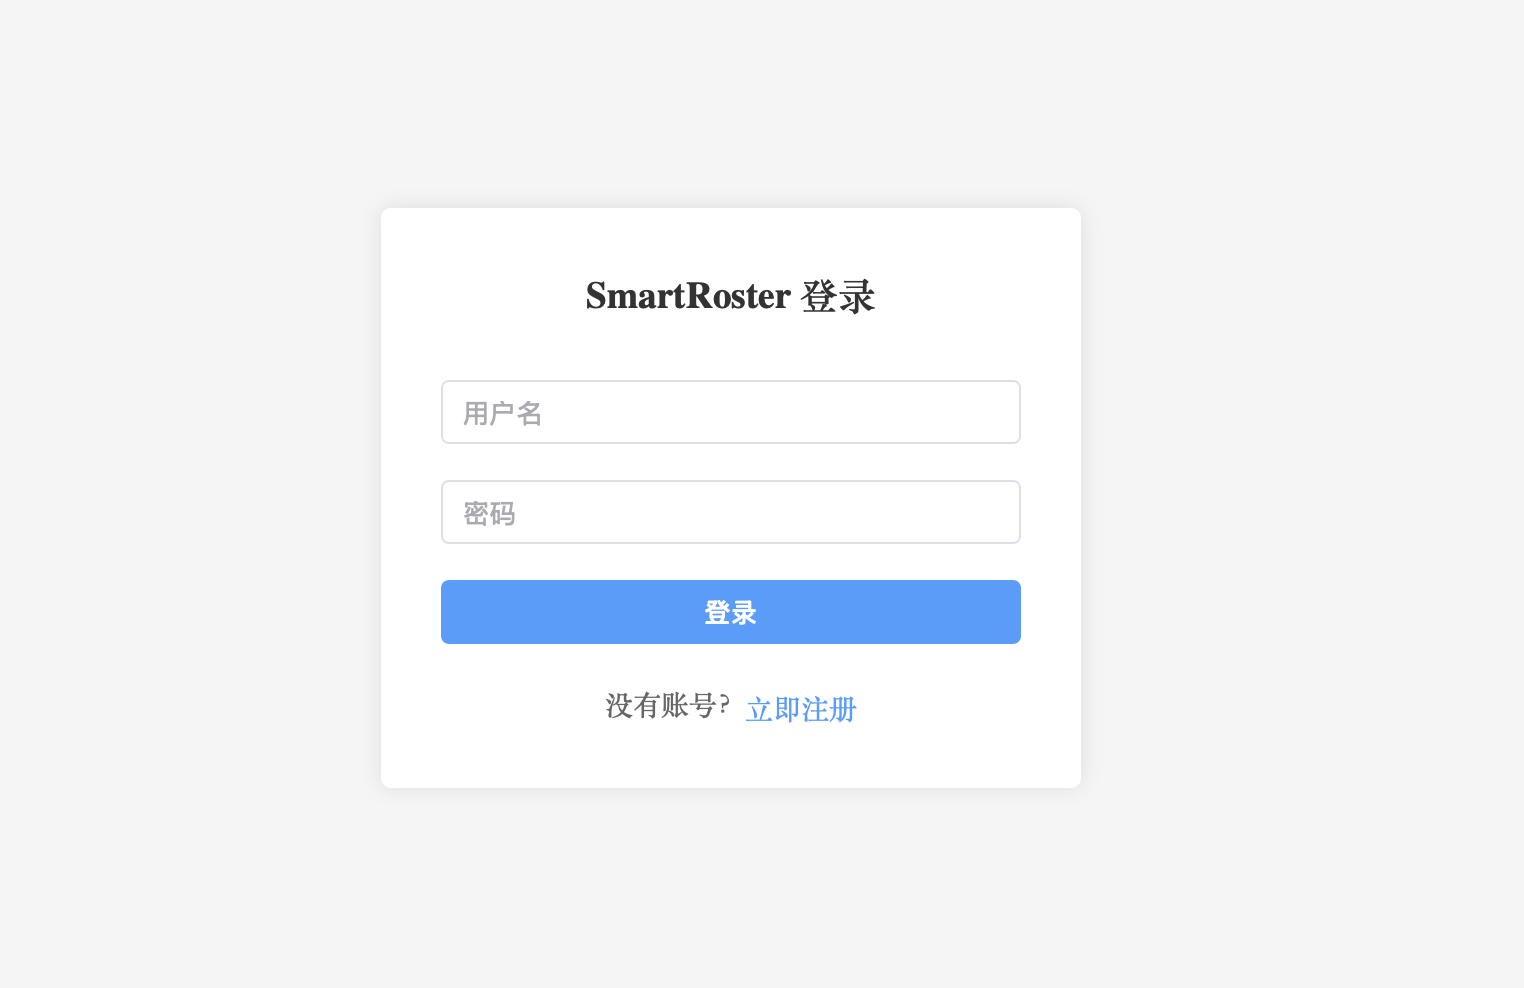
\includegraphics[width=0.8\linewidth]{./source/登录界面.png}
    \caption{登录界面}
    \label{fig:microservice-arch}
\end{figure}
\begin{figure}[H]
    \centering
    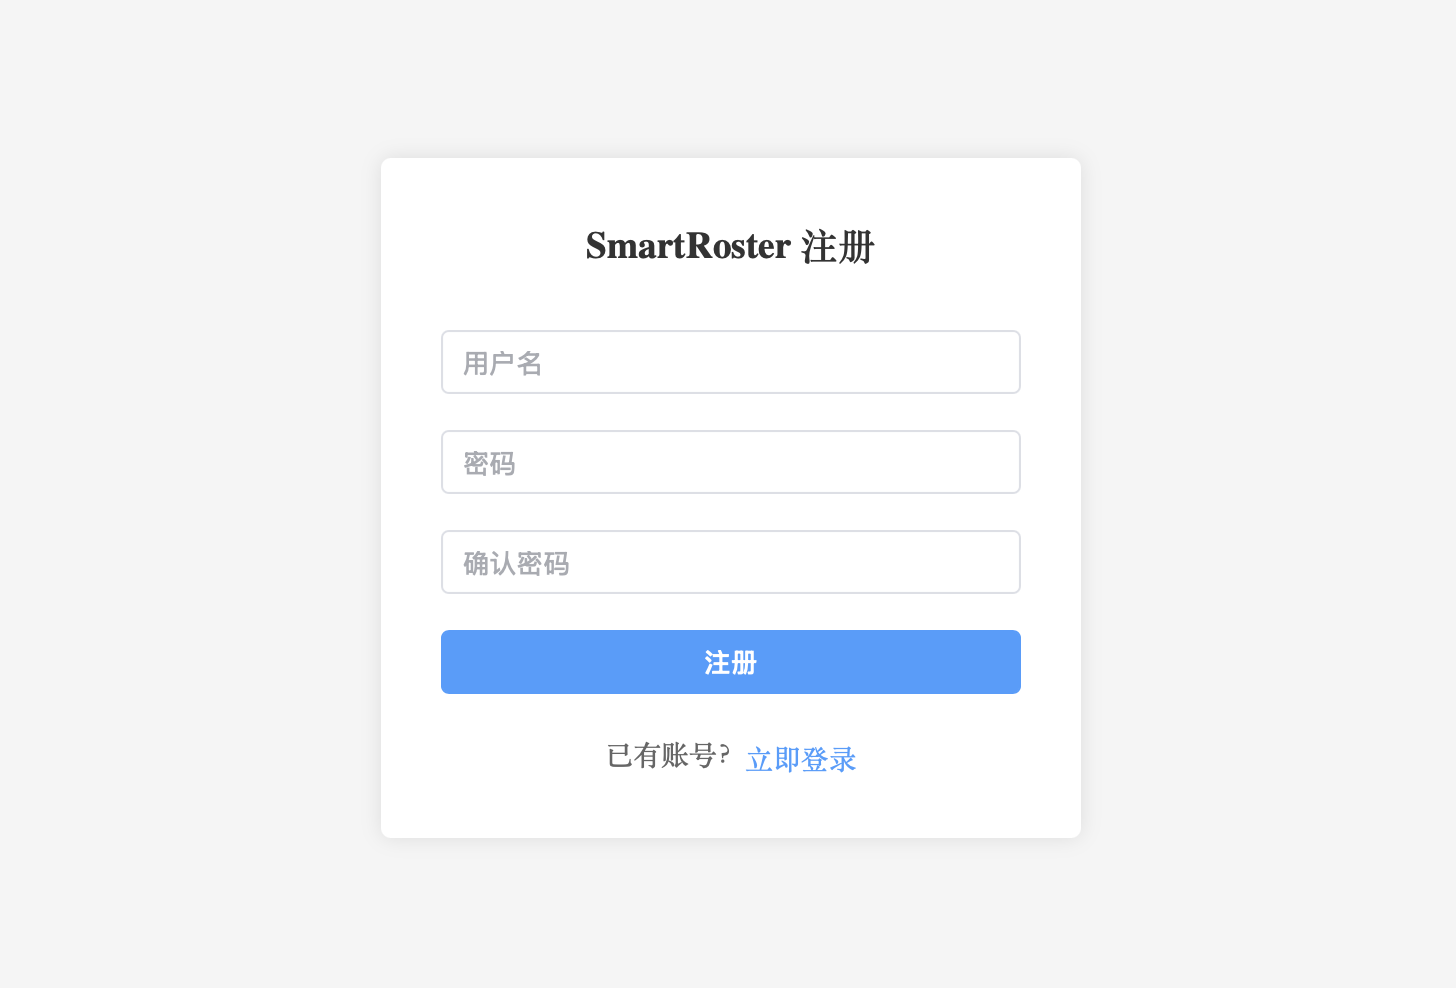
\includegraphics[width=0.8\linewidth]{./source/注册界面.png}
    \caption{注册界面}
    \label{fig:microservice-arch}
\end{figure}
\begin{figure}[H]
    \centering
    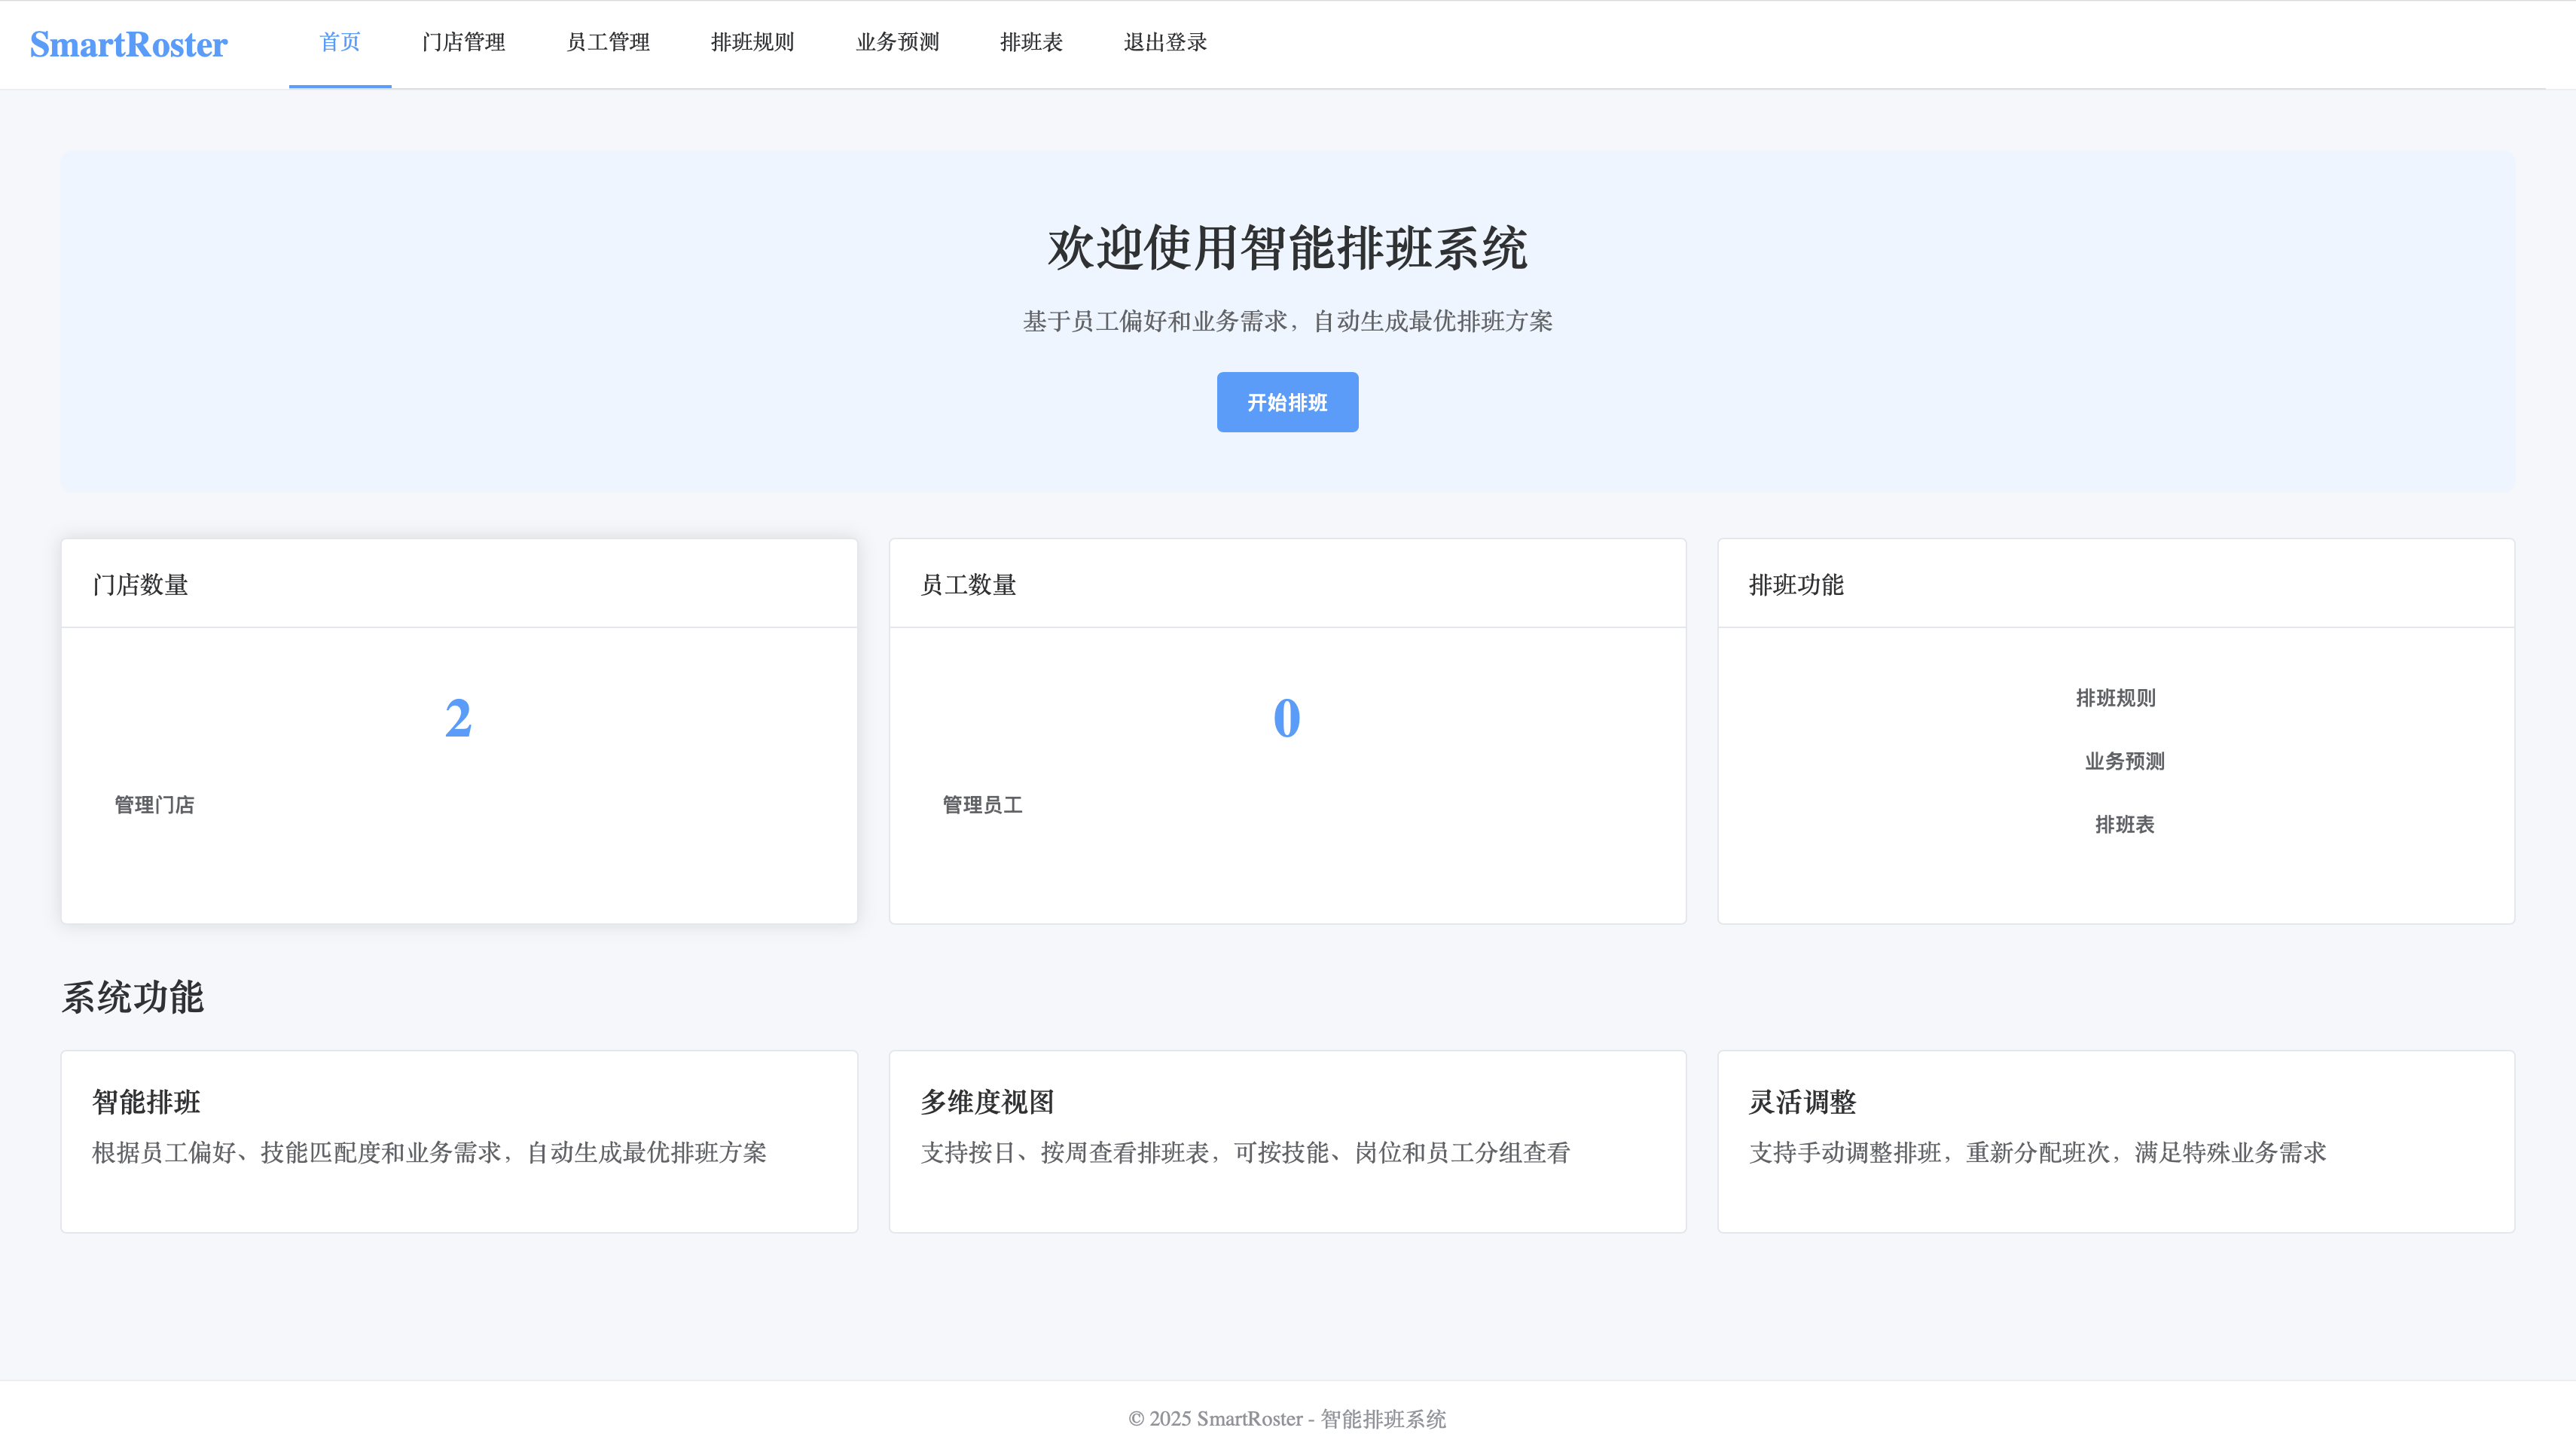
\includegraphics[width=0.8\linewidth]{./source/主页.png}
    \caption{主页}
    \label{fig:microservice-arch}
\end{figure}
\begin{figure}[H]
    \centering
    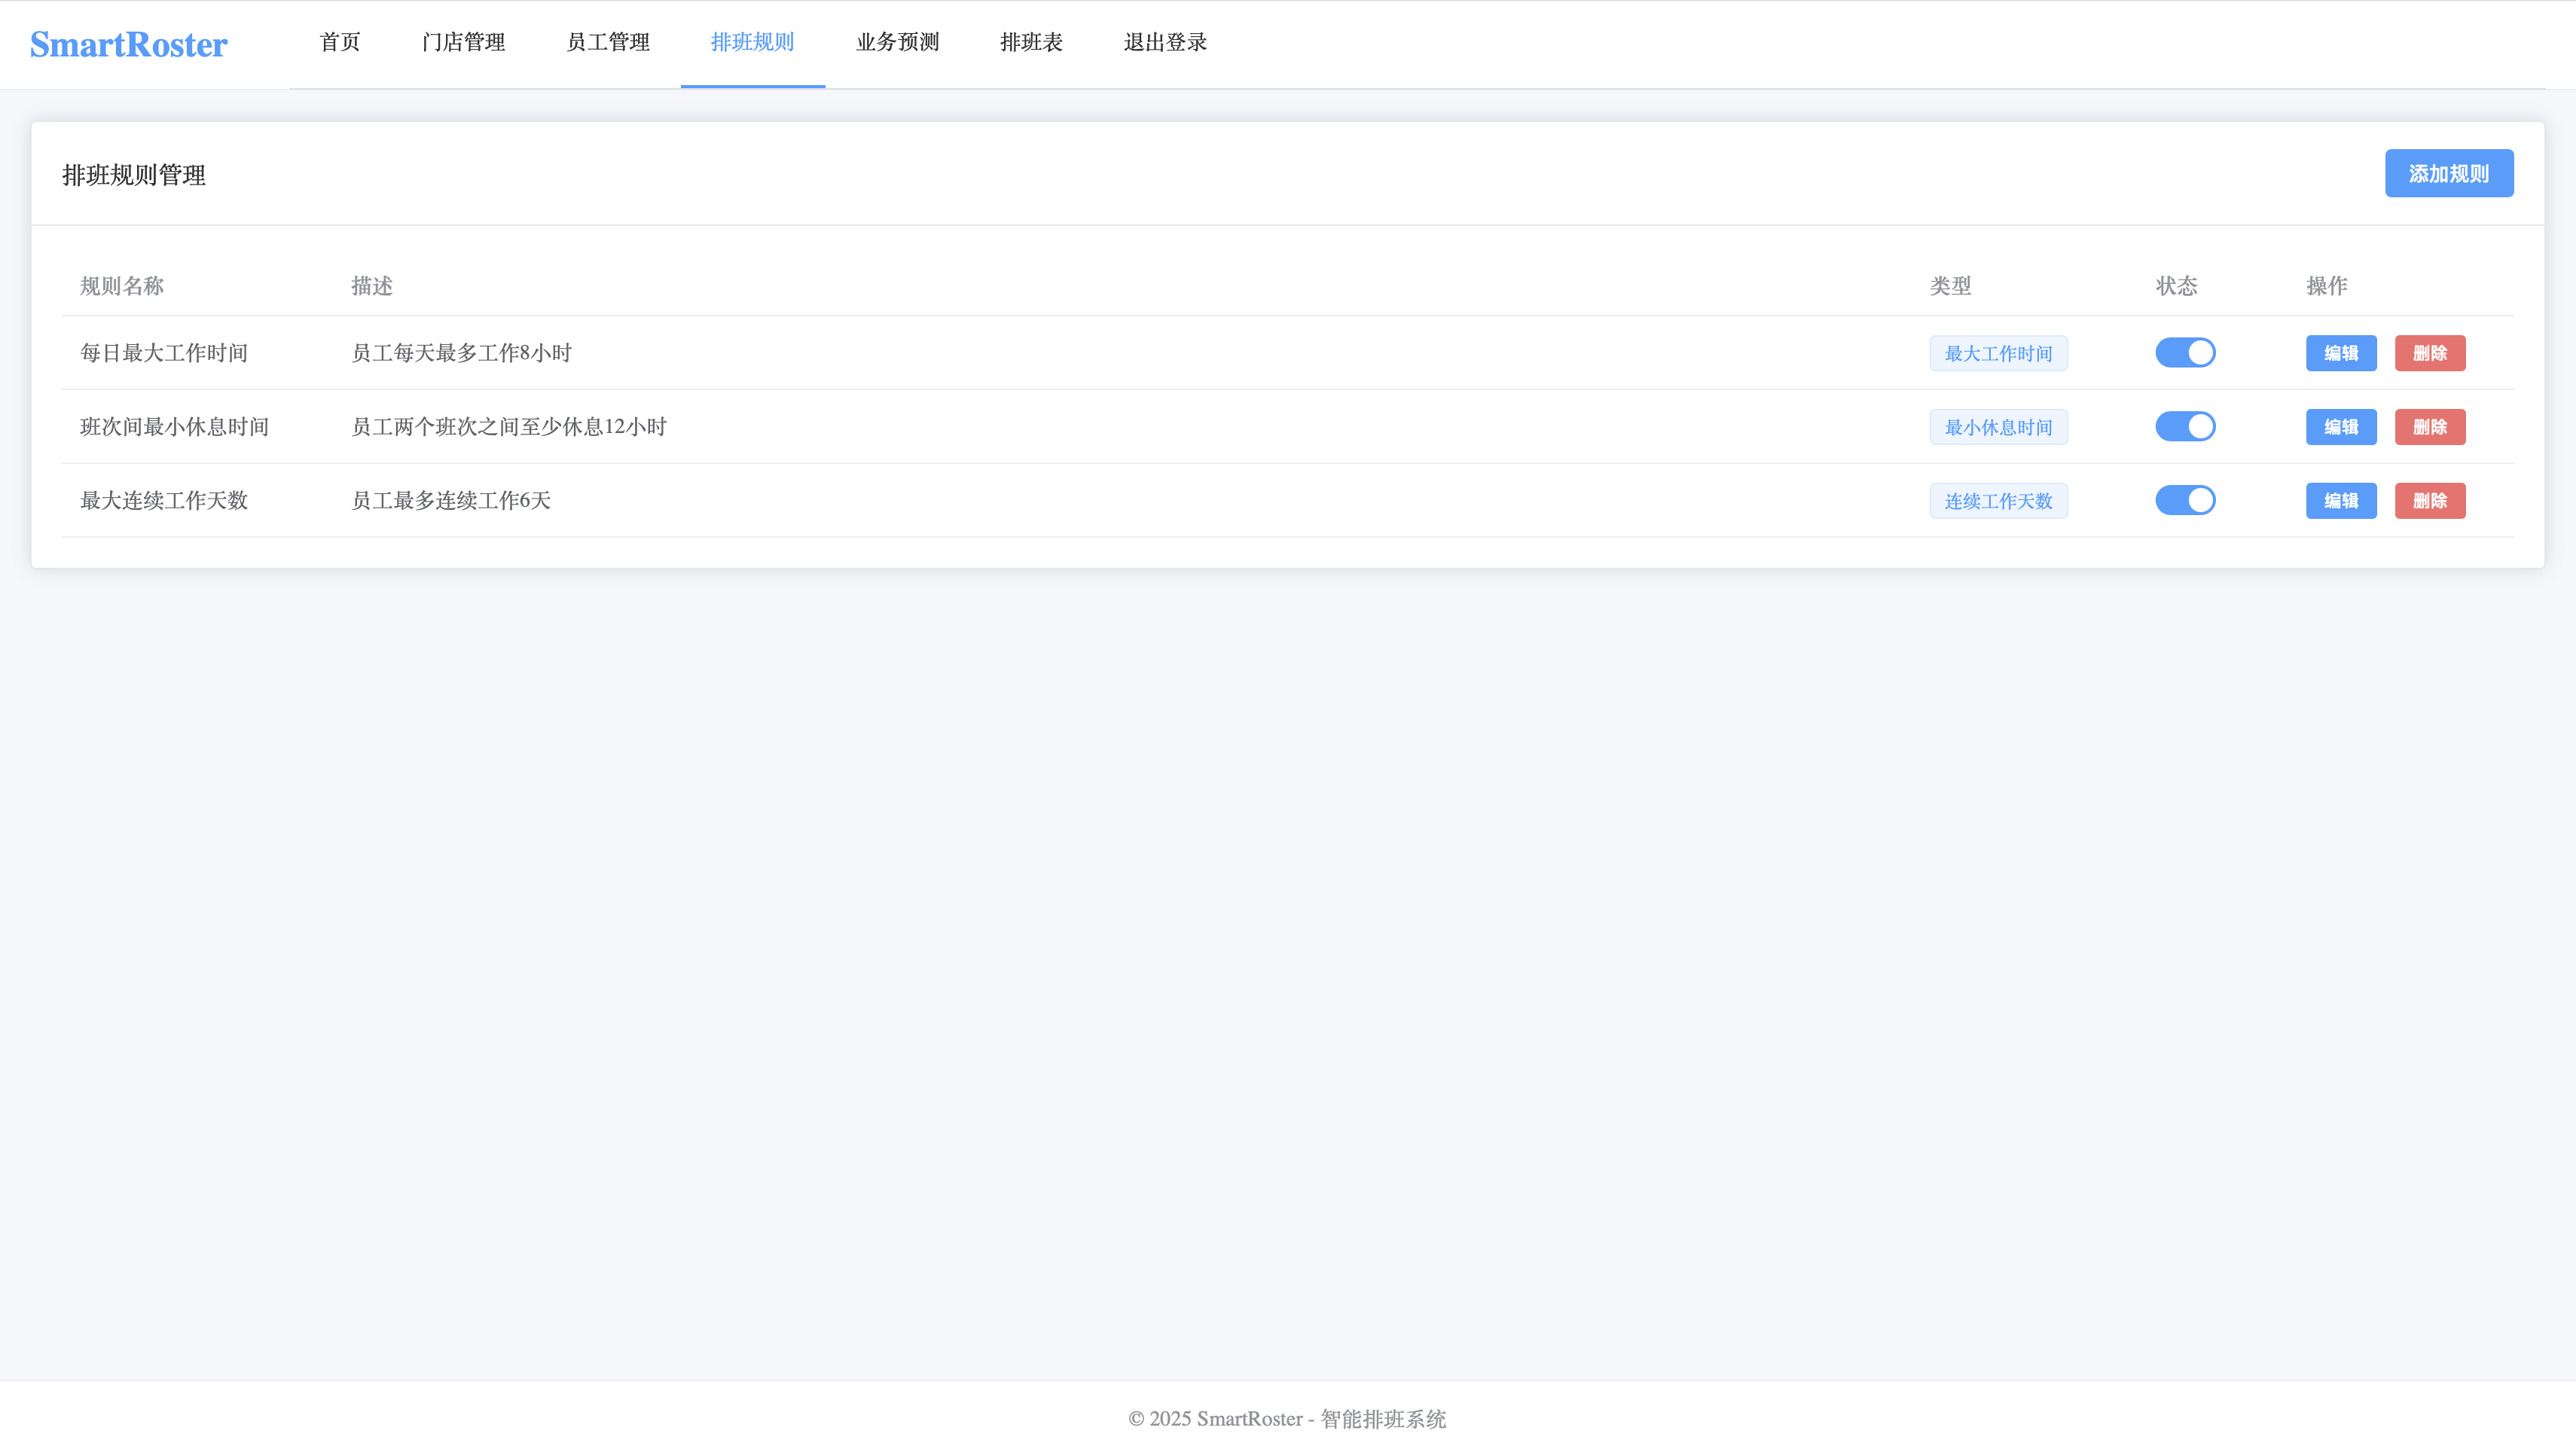
\includegraphics[width=0.8\linewidth]{./source/排班规则管理.png}
    \caption{排班规则管理}
    \label{fig:microservice-arch}
\end{figure}




\section{结论}
本文设计并实现了一套基于模拟退火算法的智能排班系统,针对零售行业排班场景中的复杂约束条件,提出了完整的解决方案。系统采用前后端分离架构与微服务技术,实现了员工管理、门店配置、智能排班等核心功能模块。通过模拟退火算法优化排班方案,在保证合规性的同时兼顾员工偏好,显著提升了排班效率。实际测试表明,系统能够快速生成高质量排班方案,有效降低人力成本并提高员工满意度。未来可进一步扩展预测算法精度和多目标优化能力,以适应更复杂的商业场景需求。

% 致谢
\section*{致谢}
\addcontentsline{toc}{section}{致谢}
% 这里添加致谢内容

% 参考文献
\section*{参考文献}
\addcontentsline{toc}{section}{参考文献}
[1]潘云龙.基于遗传算法的地铁智能排班系统设计与实现[D].华南理工大学,2013.

[2]林畅.基于B/S的银行弹性排班管理系统设计与实现[D].吉林大学,2015.

[3]熊静.基于改进遗传算法的机场AOC人员智能排班研究[D].中国民用航空飞行学院,2022.DOI:10.27722/d.cnki.gzgmh.2022.000148.

% 附录
\appendix
\addcontentsline{toc}{section}{附录A:系统功能模块详细说明}
% 这里添加附录内容

\addcontentsline{toc}{section}{附录B:核心算法伪代码}
% 这里添加附录内容
\end{document}
